\documentclass[nooutcomes]{ximera}

\graphicspath{
  {./}
  {1-1QuantitativeReasoning/}
  {1-2RelationsAndGraphs/}
  {1-3ChangingInTandem/}
  {2-1LinearEquations/}
  {2-2LinearModeling/}
  {2-3ExponentialModeling/}
  {3-1WhatIsAFunction/}
  {3-2FunctionProperties/}
  {3-3AverageRatesOfChange/}
  {4-1BuildingNewFunctions/}
  {4-2Polynomials/}
  {5-1RationalFunctions/}
   {5-2ExponentialFunctions/}
  {6-1Domain/}
  {6-2Range/}
  {6-3CompositionOfFunctions/}
  {6-4FunctionTransformations/}
  {7-1ZerosOfFunctions/}
  {7-XZerosOfPolynomials/}
  {7-2ZerosOfFamousFunctions/}
  {8-1SystemsOfEquations/}
  {6-5FunctionTransformationsProject/}
  {1-1QuantitativeReasoning/exercises/}
  {1-2RelationsAndGraphs/exercises/}
  {../1-3ChangingInTandem/exercises/}
  {../2-1LinearEquations/exercises/}
  {../2-2LinearModeling/exercises/}
  {../2-3ExponentialModeling/exercises/}
  {../3-1WhatIsAFunction/exercises/}
  {../3-2FunctionProperties/exercises/}
  {../3-3AverageRatesOfChange/exercises/}
  {../5-2ExponentialFunctions/exercises/}
  {../4-1BuildingNewFunctions/exercises/}
  {../4-2Polynomials/exercises/}
  {../5-1RationalFunctions/exercises/}
  {../6-1Domain/exercises/}
  {../6-2Range/exercises/}
  {../6-3CompositionOfFunctions/exercises/}
  {../7-1ZerosOfFunctions/exercises/}
  {../7-XZerosOfPolynomials/exercises/}
  {../7-2ZerosOfFamousFunctions/exercises/}
  {../6-4FunctionTransformations/exercises/}
  {../8-1SystemsOfEquations/exercises/}
  {../6-3FunctionTransformationsProject/exercises/}
}

\DeclareGraphicsExtensions{.pdf,.png,.jpg,.eps}

\newcommand{\mooculus}{\textsf{\textbf{MOOC}\textnormal{\textsf{ULUS}}}}

\usepackage[makeroom]{cancel} %% for strike outs

\ifxake
\else
\usepackage[most]{tcolorbox}
\fi


%\typeout{************************************************}
%\typeout{New Environments}
%\typeout{************************************************}

%% to fix for web can be removed when deployed offically with ximera2
\let\image\relax\let\endimage\relax
\NewEnviron{image}{% 
  \begin{center}\BODY\end{center}% center
}



\NewEnviron{folder}{
      \addcontentsline{toc}{section}{\textbf{\BODY}}
}

\ifxake
\let\summary\relax
\let\endsummary\relax
\newtheorem*{summary}{Summary}
\newtheorem*{callout}{Callout}
\newtheorem*{overview}{Overview}
\newtheorem*{objectives}{Objectives}
\newtheorem*{motivatingQuestions}{Motivating Questions}
\newtheorem*{MM}{Metacognitive Moment}
      
%% NEEDED FOR XIMERA 2
%\ximerizedEnvironment{summary}
%\ximerizedEnvironment{callout}
%\ximerizedEnvironment{overview} 
%\ximerizedEnvironment{objectives}
%\ximerizedEnvironment{motivatingQuestions}
%\ximerizedEnvironment{MM}
\else
%% CALLOUT
\NewEnviron{callout}{
  \begin{tcolorbox}[colback=blue!5, breakable,pad at break*=1mm]
      \BODY
  \end{tcolorbox}
}
%% MOTIVATING QUESTIONS
\NewEnviron{motivatingQuestions}{
  \begin{tcolorbox}[ breakable,pad at break*=1mm]
    \textbf{\Large Motivating Questions}\hfill
    %\begin{itemize}[label=\textbullet]
      \BODY
    %\end{itemize}
  \end{tcolorbox}
}
%% OBJECTIVES
\NewEnviron{objectives}{  
    \vspace{.5in}
      %\begin{tcolorbox}[colback=orange!5, breakable,pad at break*=1mm]
    \textbf{\Large Learning Objectives}
    \begin{itemize}[label=\textbullet]
      \BODY
    \end{itemize}
    %\end{tcolorbox}
}
%% DEFINITION
\let\definition\relax
\let\enddefinition\relax
\NewEnviron{definition}{
  \begin{tcolorbox}[ breakable,pad at break*=1mm]
    \noindent\textbf{Definition}~
      \BODY
  \end{tcolorbox}
}
%% OVERVIEW
\let\overview\relax
\let\overview\relax
\NewEnviron{overview}{
  \begin{tcolorbox}[ breakable,pad at break*=1mm]
    \textbf{\Large Overview}
    %\begin{itemize}[label=\textbullet] %% breaks Xake
      \BODY
    %\end{itemize}
  \end{tcolorbox}
}
%% SUMMARY
\let\summary\relax
\let\endsummary\relax
\NewEnviron{summary}{
  \begin{tcolorbox}[ breakable,pad at break*=1mm]
    \textbf{\Large Summary}
    %\begin{itemize}[label=\textbullet] %% breaks Xake
      \BODY
    %\end{itemize}
  \end{tcolorbox}
}
%% REMARK
\let\remark\relax
\let\endremark\relax
\NewEnviron{remark}{
  \begin{tcolorbox}[colback=green!5, breakable,pad at break*=1mm]
    \noindent\textbf{Remark}~
      \BODY
  \end{tcolorbox}
}
%% EXPLANATION
\let\explanation\relax
\let\endexplanation\relax
\NewEnviron{explanation}{
    \normalfont
    \noindent\textbf{Explanation}~
      \BODY
}
%% EXPLORATION
\let\exploration\relax
\let\endexploration\relax
\NewEnviron{exploration}{
  \begin{tcolorbox}[colback=yellow!10, breakable,pad at break*=1mm]
    \noindent\textbf{Exploration}~
      \BODY
  \end{tcolorbox}
}
%% METACOGNITIVE MOMENTS
\let\MM\relax
\let\endMM\relax
\NewEnviron{MM}{
  \begin{tcolorbox}[colback=pink!15, breakable,pad at break*=1mm]
    \noindent\textbf{Metacognitive Moment}~
      \BODY
  \end{tcolorbox}
}


\fi





%Notes on what envirnoment to use:  Example with Explanation in text; if they are supposed to answer- Problem; no answer - Exploration


%\typeout{************************************************}
%% Header and footers
%\typeout{************************************************}

\newcommand{\licenseAcknowledgement}{Licensed under Creative Commons 4.0}
\newcommand{\licenseAPC}{\renewcommand{\licenseAcknowledgement}{\textbf{Acknowledgements:} Active Prelude to Calculus (https://activecalculus.org/prelude) }}
\newcommand{\licenseSZ}{\renewcommand{\licenseAcknowledgement}{\textbf{Acknowledgements:} Stitz Zeager Open Source Mathematics (https://www.stitz-zeager.com/) }}
\newcommand{\licenseAPCSZ}{\renewcommand{\licenseAcknowledgement}{\textbf{Acknowledgements:} Active Prelude to Calculus (https://activecalculus.org/prelude) and Stitz Zeager Open Source Mathematics (https://www.stitz-zeager.com/) }}
\newcommand{\licenseORCCA}{\renewcommand{\licenseAcknowledgement}{\textbf{Acknowledgements:}Original source material, products with readable and accessible
math content, and other information freely available at pcc.edu/orcca.}}
\newcommand{\licenseY}{\renewcommand{\licenseAcknowledgement}{\textbf{Acknowledgements:} Yoshiwara Books (https://yoshiwarabooks.org/)}}
\newcommand{\licenseOS}{\renewcommand{\licenseAcknowledgement}{\textbf{Acknowledgements:} OpenStax College Algebra (https://openstax.org/details/books/college-algebra)}}
\newcommand{\licenseAPCSZCSCC}{\renewcommand{\licenseAcknowledgement}{\textbf{Acknowledgements:} Active Prelude to Calculus (https://activecalculus.org/prelude), Stitz Zeager Open Source Mathematics (https://www.stitz-zeager.com/), CSCC PreCalculus and Calculus texts (https://ximera.osu.edu/csccmathematics)}}

\ifxake\else %% do nothing on the website
\usepackage{fancyhdr}
\pagestyle{fancy}
\fancyhf{}
\fancyhead[R]{\sectionmark}
\fancyfoot[L]{\thepage}
\fancyfoot[C]{\licenseAcknowledgement}
\renewcommand{\headrulewidth}{0pt}
\renewcommand{\footrulewidth}{0pt}
\fi

%%%%%%%%%%%%%%%%



%\typeout{************************************************}
%\typeout{Table of Contents}
%\typeout{************************************************}


%% Edit this to change the font style
\newcommand{\sectionHeadStyle}{\sffamily\bfseries}


\makeatletter

%% part uses arabic numerals
\renewcommand*\thepart{\arabic{part}}


\ifxake\else
\renewcommand\chapterstyle{%
  \def\maketitle{%
    \addtocounter{titlenumber}{1}%
    \pagestyle{fancy}
    \phantomsection
    \addcontentsline{toc}{section}{\textbf{\thepart.\thetitlenumber\hspace{1em}\@title}}%
                    {\flushleft\small\sectionHeadStyle\@pretitle\par\vspace{-1.5em}}%
                    {\flushleft\LARGE\sectionHeadStyle\thepart.\thetitlenumber\hspace{1em}\@title \par }%
                    {\setcounter{problem}{0}\setcounter{sectiontitlenumber}{0}}%
                    \par}}





\renewcommand\sectionstyle{%
  \def\maketitle{%
    \addtocounter{sectiontitlenumber}{1}
    \pagestyle{fancy}
    \phantomsection
    \addcontentsline{toc}{subsection}{\thepart.\thetitlenumber.\thesectiontitlenumber\hspace{1em}\@title}%
    {\flushleft\small\sectionHeadStyle\@pretitle\par\vspace{-1.5em}}%
    {\flushleft\Large\sectionHeadStyle\thepart.\thetitlenumber.\thesectiontitlenumber\hspace{1em}\@title \par}%
    %{\setcounter{subsectiontitlenumber}{0}}%
    \par}}



\renewcommand\section{\@startsection{paragraph}{10}{\z@}%
                                     {-3.25ex\@plus -1ex \@minus -.2ex}%
                                     {1.5ex \@plus .2ex}%
                                     {\normalfont\large\sectionHeadStyle}}
\renewcommand\subsection{\@startsection{subparagraph}{10}{\z@}%
                                    {3.25ex \@plus1ex \@minus.2ex}%
                                    {-1em}%
                                    {\normalfont\normalsize\sectionHeadStyle}}

\fi

%% redefine Part
\renewcommand\part{%
   {\setcounter{titlenumber}{0}}
  \if@openright
    \cleardoublepage
  \else
    \clearpage
  \fi
  \thispagestyle{plain}%
  \if@twocolumn
    \onecolumn
    \@tempswatrue
  \else
    \@tempswafalse
  \fi
  \null\vfil
  \secdef\@part\@spart}

\def\@part[#1]#2{%
    \ifnum \c@secnumdepth >-2\relax
      \refstepcounter{part}%
      \addcontentsline{toc}{part}{\thepart\hspace{1em}#1}%
    \else
      \addcontentsline{toc}{part}{#1}%
    \fi
    \markboth{}{}%
    {\centering
     \interlinepenalty \@M
     \normalfont
     \ifnum \c@secnumdepth >-2\relax
       \huge\sffamily\bfseries \partname\nobreakspace\thepart
       \par
       \vskip 20\p@
     \fi
     \Huge \bfseries #2\par}%
    \@endpart}
\def\@spart#1{%
    {\centering
     \interlinepenalty \@M
     \normalfont
     \Huge \bfseries #1\par}%
    \@endpart}
\def\@endpart{\vfil\newpage
              \if@twoside
               \if@openright
                \null
                \thispagestyle{empty}%
                \newpage
               \fi
              \fi
              \if@tempswa
                \twocolumn
                \fi}



\makeatother





%\typeout{************************************************}
%\typeout{Stuff from Ximera}
%\typeout{************************************************}



\usepackage{array}  %% This is for typesetting long division
\setlength{\extrarowheight}{+.1cm}
\newdimen\digitwidth
\settowidth\digitwidth{9}
\def\divrule#1#2{
\noalign{\moveright#1\digitwidth
\vbox{\hrule width#2\digitwidth}}}





\newcommand{\RR}{\mathbb R}
\newcommand{\R}{\mathbb R}
\newcommand{\N}{\mathbb N}
\newcommand{\Z}{\mathbb Z}

\newcommand{\sagemath}{\textsf{SageMath}}


\def\d{\,d}
%\renewcommand{\d}{\mathop{}\!d}
\newcommand{\dd}[2][]{\frac{\d #1}{\d #2}}
\newcommand{\pp}[2][]{\frac{\partial #1}{\partial #2}}
\renewcommand{\l}{\ell}
\newcommand{\ddx}{\frac{d}{\d x}}



%\newcommand{\unit}{\,\mathrm}
\newcommand{\unit}{\mathop{}\!\mathrm}
\newcommand{\eval}[1]{\bigg[ #1 \bigg]}
\newcommand{\seq}[1]{\left( #1 \right)}
\renewcommand{\epsilon}{\varepsilon}
\renewcommand{\phi}{\varphi}


\renewcommand{\iff}{\Leftrightarrow}

\DeclareMathOperator{\arccot}{arccot}
\DeclareMathOperator{\arcsec}{arcsec}
\DeclareMathOperator{\arccsc}{arccsc}
\DeclareMathOperator{\sign}{sign}


%\DeclareMathOperator{\divergence}{divergence}
%\DeclareMathOperator{\curl}[1]{\grad\cross #1}
\newcommand{\lto}{\mathop{\longrightarrow\,}\limits}

\renewcommand{\bar}{\overline}

\colorlet{textColor}{black}
\colorlet{background}{white}
\colorlet{penColor}{blue!50!black} % Color of a curve in a plot
\colorlet{penColor2}{red!50!black}% Color of a curve in a plot
\colorlet{penColor3}{red!50!blue} % Color of a curve in a plot
\colorlet{penColor4}{green!50!black} % Color of a curve in a plot
\colorlet{penColor5}{orange!80!black} % Color of a curve in a plot
\colorlet{penColor6}{yellow!70!black} % Color of a curve in a plot
\colorlet{fill1}{penColor!20} % Color of fill in a plot
\colorlet{fill2}{penColor2!20} % Color of fill in a plot
\colorlet{fillp}{fill1} % Color of positive area
\colorlet{filln}{penColor2!20} % Color of negative area
\colorlet{fill3}{penColor3!20} % Fill
\colorlet{fill4}{penColor4!20} % Fill
\colorlet{fill5}{penColor5!20} % Fill
\colorlet{gridColor}{gray!50} % Color of grid in a plot

\newcommand{\surfaceColor}{violet}
\newcommand{\surfaceColorTwo}{redyellow}
\newcommand{\sliceColor}{greenyellow}




\pgfmathdeclarefunction{gauss}{2}{% gives gaussian
  \pgfmathparse{1/(#2*sqrt(2*pi))*exp(-((x-#1)^2)/(2*#2^2))}%
}





%\typeout{************************************************}
%\typeout{ORCCA Preamble.Tex}
%\typeout{************************************************}


%% \usepackage{geometry}
%% \geometry{letterpaper,total={408pt,9.0in}}
%% Custom Page Layout Adjustments (use latex.geometry)
%% \usepackage{amsmath,amssymb}
%% \usepackage{pgfplots}
\usepackage{pifont}                                         %needed for symbols, s.a. airplane symbol
\usetikzlibrary{positioning,fit,backgrounds}                %needed for nested diagrams
\usetikzlibrary{calc,trees,positioning,arrows,fit,shapes}   %needed for set diagrams
\usetikzlibrary{decorations.text}                           %needed for text following a curve
\usetikzlibrary{arrows,arrows.meta}                         %needed for open/closed intervals
\usetikzlibrary{positioning,3d,shapes.geometric}            %needed for 3d number sets tower

%% NEEDED FOR XIMERA 1
%\usetkzobj{all}       %NO LONGER VALID
%%%%%%%%%%%%%%

\usepackage{tikz-3dplot}
\usepackage{tkz-euclide}                     %needed for triangle diagrams
\usepgfplotslibrary{fillbetween}                            %shade regions of a plot
\usetikzlibrary{shadows}                                    %function diagrams
\usetikzlibrary{positioning}                                %function diagrams
\usetikzlibrary{shapes}                                     %function diagrams
%%% global colors from https://www.pcc.edu/web-services/style-guide/basics/color/ %%%
\definecolor{ruby}{HTML}{9E0C0F}
\definecolor{turquoise}{HTML}{008099}
\definecolor{emerald}{HTML}{1c8464}
\definecolor{amber}{HTML}{c7502a}
\definecolor{amethyst}{HTML}{70485b}
\definecolor{sapphire}{HTML}{263c53}
\colorlet{firstcolor}{sapphire}
\colorlet{secondcolor}{turquoise}
\colorlet{thirdcolor}{emerald}
\colorlet{fourthcolor}{amber}
\colorlet{fifthcolor}{amethyst}
\colorlet{sixthcolor}{ruby}
\colorlet{highlightcolor}{green!50!black}
\colorlet{graphbackground}{white}
\colorlet{wood}{brown!60!white}
%%% curve, dot, and graph custom styles %%%
\pgfplotsset{firstcurve/.style      = {color=firstcolor,  mark=none, line width=1pt, {Kite}-{Kite}, solid}}
\pgfplotsset{secondcurve/.style     = {color=secondcolor, mark=none, line width=1pt, {Kite}-{Kite}, solid}}
\pgfplotsset{thirdcurve/.style      = {color=thirdcolor,  mark=none, line width=1pt, {Kite}-{Kite}, solid}}
\pgfplotsset{fourthcurve/.style     = {color=fourthcolor, mark=none, line width=1pt, {Kite}-{Kite}, solid}}
\pgfplotsset{fifthcurve/.style      = {color=fifthcolor,  mark=none, line width=1pt, {Kite}-{Kite}, solid}}
\pgfplotsset{highlightcurve/.style  = {color=highlightcolor,  mark=none, line width=5pt, -, opacity=0.3}}   % thick, opaque curve for highlighting
\pgfplotsset{asymptote/.style       = {color=gray, mark=none, line width=1pt, <->, dashed}}
\pgfplotsset{symmetryaxis/.style    = {color=gray, mark=none, line width=1pt, <->, dashed}}
\pgfplotsset{guideline/.style       = {color=gray, mark=none, line width=1pt, -}}
\tikzset{guideline/.style           = {color=gray, mark=none, line width=1pt, -}}
\pgfplotsset{altitude/.style        = {dashed, color=gray, thick, mark=none, -}}
\tikzset{altitude/.style            = {dashed, color=gray, thick, mark=none, -}}
\pgfplotsset{radius/.style          = {dashed, thick, mark=none, -}}
\tikzset{radius/.style              = {dashed, thick, mark=none, -}}
\pgfplotsset{rightangle/.style      = {color=gray, mark=none, -}}
\tikzset{rightangle/.style          = {color=gray, mark=none, -}}
\pgfplotsset{closedboundary/.style  = {color=black, mark=none, line width=1pt, {Kite}-{Kite},solid}}
\tikzset{closedboundary/.style      = {color=black, mark=none, line width=1pt, {Kite}-{Kite},solid}}
\pgfplotsset{openboundary/.style    = {color=black, mark=none, line width=1pt, {Kite}-{Kite},dashed}}
\tikzset{openboundary/.style        = {color=black, mark=none, line width=1pt, {Kite}-{Kite},dashed}}
\tikzset{verticallinetest/.style    = {color=gray, mark=none, line width=1pt, <->,dashed}}
\pgfplotsset{soliddot/.style        = {color=firstcolor,  mark=*, only marks}}
\pgfplotsset{hollowdot/.style       = {color=firstcolor,  mark=*, only marks, fill=graphbackground}}
\pgfplotsset{blankgraph/.style      = {xmin=-10, xmax=10,
                                        ymin=-10, ymax=10,
                                        axis line style={-, draw opacity=0 },
                                        axis lines=box,
                                        major tick length=0mm,
                                        xtick={-10,-9,...,10},
                                        ytick={-10,-9,...,10},
                                        grid=major,
                                        grid style={solid,gray!20},
                                        xticklabels={,,},
                                        yticklabels={,,},
                                        minor xtick=,
                                        minor ytick=,
                                        xlabel={},ylabel={},
                                        width=0.75\textwidth,
                                      }
            }
\pgfplotsset{numberline/.style      = {xmin=-10,xmax=10,
                                        minor xtick={-11,-10,...,11},
                                        xtick={-10,-5,...,10},
                                        every tick/.append style={thick},
                                        axis y line=none,
                                        y=15pt,
                                        axis lines=middle,
                                        enlarge x limits,
                                        grid=none,
                                        clip=false,
                                        axis background/.style={},
                                        after end axis/.code={
                                          \path (axis cs:0,0)
                                          node [anchor=north,yshift=-0.075cm] {\footnotesize 0};
                                        },
                                        every axis x label/.style={at={(current axis.right of origin)},anchor=north},
                                      }
            }
\pgfplotsset{openinterval/.style={color=firstcolor,mark=none,ultra thick,{Parenthesis}-{Parenthesis}}}
\pgfplotsset{openclosedinterval/.style={color=firstcolor,mark=none,ultra thick,{Parenthesis}-{Bracket}}}
\pgfplotsset{closedinterval/.style={color=firstcolor,mark=none,ultra thick,{Bracket}-{Bracket}}}
\pgfplotsset{closedopeninterval/.style={color=firstcolor,mark=none,ultra thick,{Bracket}-{Parenthesis}}}
\pgfplotsset{infiniteopeninterval/.style={color=firstcolor,mark=none,ultra thick,{Kite}-{Parenthesis}}}
\pgfplotsset{openinfiniteinterval/.style={color=firstcolor,mark=none,ultra thick,{Parenthesis}-{Kite}}}
\pgfplotsset{infiniteclosedinterval/.style={color=firstcolor,mark=none,ultra thick,{Kite}-{Bracket}}}
\pgfplotsset{closedinfiniteinterval/.style={color=firstcolor,mark=none,ultra thick,{Bracket}-{Kite}}}
\pgfplotsset{infiniteinterval/.style={color=firstcolor,mark=none,ultra thick,{Kite}-{Kite}}}
\pgfplotsset{interval/.style= {ultra thick, -}}
%%% cycle list of plot styles for graphs with multiple plots %%%
\pgfplotscreateplotcyclelist{pccstylelist}{%
  firstcurve\\%
  secondcurve\\%
  thirdcurve\\%
  fourthcurve\\%
  fifthcurve\\%
}
%%% default plot settings %%%
\pgfplotsset{every axis/.append style={
  axis x line=middle,    % put the x axis in the middle
  axis y line=middle,    % put the y axis in the middle
  axis line style={<->}, % arrows on the axis
  scaled ticks=false,
  tick label style={/pgf/number format/fixed},
  xlabel={$x$},          % default put x on x-axis
  ylabel={$y$},          % default put y on y-axis
  xmin = -7,xmax = 7,    % most graphs have this window
  ymin = -7,ymax = 7,    % most graphs have this window
  domain = -7:7,
  xtick = {-6,-4,...,6}, % label these ticks
  ytick = {-6,-4,...,6}, % label these ticks
  yticklabel style={inner sep=0.333ex},
  minor xtick = {-7,-6,...,7}, % include these ticks, some without label
  minor ytick = {-7,-6,...,7}, % include these ticks, some without label
  scale only axis,       % don't consider axis and tick labels for width and height calculation
  cycle list name=pccstylelist,
  tick label style={font=\footnotesize},
  legend cell align=left,
  grid = both,
  grid style = {solid,gray!20},
  axis background/.style={fill=graphbackground},
}}
\pgfplotsset{framed/.style={axis background/.style ={draw=gray}}}
%\pgfplotsset{framed/.style={axis background/.style ={draw=gray,fill=graphbackground,rounded corners=3ex}}}
%%% other tikz (not pgfplots) settings %%%
%\tikzset{axisnode/.style={font=\scriptsize,text=black}}
\tikzset{>=stealth}
%%% for nested diagram in types of numbers section %%%
\newcommand\drawnestedsets[4]{
  \def\position{#1}             % initial position
  \def\nbsets{#2}               % number of sets
  \def\listofnestedsets{#3}     % list of sets
  \def\reversedlistofcolors{#4} % reversed list of colors
  % position and draw labels of sets
  \coordinate (circle-0) at (#1);
  \coordinate (set-0) at (#1);
  \foreach \set [count=\c] in \listofnestedsets {
    \pgfmathtruncatemacro{\cminusone}{\c - 1}
    % label of current set (below previous nested set)
    \node[below=3pt of circle-\cminusone,inner sep=0]
    (set-\c) {\set};
    % current set (fit current label and previous set)
    \node[circle,inner sep=0,fit=(circle-\cminusone)(set-\c)]
    (circle-\c) {};
  }
  % draw and fill sets in reverse order
  \begin{scope}[on background layer]
    \foreach \col[count=\c] in \reversedlistofcolors {
      \pgfmathtruncatemacro{\invc}{\nbsets-\c}
      \pgfmathtruncatemacro{\invcplusone}{\invc+1}
      \node[circle,draw,fill=\col,inner sep=0,
      fit=(circle-\invc)(set-\invcplusone)] {};
    }
  \end{scope}
  }
\ifdefined\tikzset
\tikzset{ampersand replacement = \amp}
\fi
\newcommand{\abs}[1]{\left\lvert#1\right\rvert}
%\newcommand{\point}[2]{\left(#1,#2\right)}
\newcommand{\highlight}[1]{\definecolor{sapphire}{RGB}{59,90,125} {\color{sapphire}{{#1}}}}
\newcommand{\firsthighlight}[1]{\definecolor{sapphire}{RGB}{59,90,125} {\color{sapphire}{{#1}}}}
\newcommand{\secondhighlight}[1]{\definecolor{emerald}{RGB}{20,97,75} {\color{emerald}{{#1}}}}
\newcommand{\unhighlight}[1]{{\color{black}{{#1}}}}
\newcommand{\lowlight}[1]{{\color{lightgray}{#1}}}
\newcommand{\attention}[1]{\mathord{\overset{\downarrow}{#1}}}
\newcommand{\nextoperation}[1]{\mathord{\boxed{#1}}}
\newcommand{\substitute}[1]{{\color{blue}{{#1}}}}
\newcommand{\pinover}[2]{\overset{\overset{\mathrm{\ #2\ }}{|}}{\strut #1 \strut}}
\newcommand{\addright}[1]{{\color{blue}{{{}+#1}}}}
\newcommand{\addleft}[1]{{\color{blue}{{#1+{}}}}}
\newcommand{\subtractright}[1]{{\color{blue}{{{}-#1}}}}
\newcommand{\multiplyright}[2][\cdot]{{\color{blue}{{{}#1#2}}}}
\newcommand{\multiplyleft}[2][\cdot]{{\color{blue}{{#2#1{}}}}}
\newcommand{\divideunder}[2]{\frac{#1}{{\color{blue}{{#2}}}}}
\newcommand{\divideright}[1]{{\color{blue}{{{}\div#1}}}}
\newcommand{\negate}[1]{{\color{blue}{{-}}}\left(#1\right)}
\newcommand{\cancelhighlight}[1]{\definecolor{sapphire}{RGB}{59,90,125}{\color{sapphire}{{\cancel{#1}}}}}
\newcommand{\secondcancelhighlight}[1]{\definecolor{emerald}{RGB}{20,97,75}{\color{emerald}{{\bcancel{#1}}}}}
\newcommand{\thirdcancelhighlight}[1]{\definecolor{amethyst}{HTML}{70485b}{\color{amethyst}{{\xcancel{#1}}}}}
\newcommand{\lt}{<} %% Bart: WHY?
\newcommand{\gt}{>} %% Bart: WHY?
\newcommand{\amp}{&} %% Bart: WHY?


%%% These commands break Xake
%% \newcommand{\apple}{\text{🍎}}
%% \newcommand{\banana}{\text{🍌}}
%% \newcommand{\pear}{\text{🍐}}
%% \newcommand{\cat}{\text{🐱}}
%% \newcommand{\dog}{\text{🐶}}

\newcommand{\apple}{PICTURE OF APPLE}
\newcommand{\banana}{PICTURE OF BANANA}
\newcommand{\pear}{PICTURE OF PEAR}
\newcommand{\cat}{PICTURE OF CAT}
\newcommand{\dog}{PICTURE OF DOG}


%%%%% INDEX STUFF
\newcommand{\dfn}[1]{\textbf{#1}\index{#1}}
\usepackage{imakeidx}
\makeindex[intoc]
\makeatletter
\gdef\ttl@savemark{\sectionmark{}}
\makeatother












 % for drawing cube in Optimization problem
\usetikzlibrary{quotes,arrows.meta}
\tikzset{
  annotated cuboid/.pic={
    \tikzset{%
      every edge quotes/.append style={midway, auto},
      /cuboid/.cd,
      #1
    }
    \draw [every edge/.append style={pic actions, densely dashed, opacity=.5}, pic actions]
    (0,0,0) coordinate (o) -- ++(-\cubescale*\cubex,0,0) coordinate (a) -- ++(0,-\cubescale*\cubey,0) coordinate (b) edge coordinate [pos=1] (g) ++(0,0,-\cubescale*\cubez)  -- ++(\cubescale*\cubex,0,0) coordinate (c) -- cycle
    (o) -- ++(0,0,-\cubescale*\cubez) coordinate (d) -- ++(0,-\cubescale*\cubey,0) coordinate (e) edge (g) -- (c) -- cycle
    (o) -- (a) -- ++(0,0,-\cubescale*\cubez) coordinate (f) edge (g) -- (d) -- cycle;
    \path [every edge/.append style={pic actions, |-|}]
    (b) +(0,-5pt) coordinate (b1) edge ["x"'] (b1 -| c)
    (b) +(-5pt,0) coordinate (b2) edge ["y"] (b2 |- a)
    (c) +(3.5pt,-3.5pt) coordinate (c2) edge ["x"'] ([xshift=3.5pt,yshift=-3.5pt]e)
    ;
  },
  /cuboid/.search also={/tikz},
  /cuboid/.cd,
  width/.store in=\cubex,
  height/.store in=\cubey,
  depth/.store in=\cubez,
  units/.store in=\cubeunits,
  scale/.store in=\cubescale,
  width=10,
  height=10,
  depth=10,
  units=cm,
  scale=.1,
}

\author{Elizabeth Miller}
\license{Creative Commons Attribution-ShareAlike 4.0 International License}
\acknowledgement{https://activecalculus.org/prelude/sec-exp-growth.html}

\title{Exponential Functions}

\begin{document}
\licenseAPC
\begin{abstract}
  
\end{abstract}
\maketitle


%\typeout{************************************************}
%\typeout{Motivating Questions}
%\typeout{************************************************}

\begin{motivatingQuestions}\begin{itemize}
\item What does it mean to say that a function is ``exponential''?
\item How much data do we need to know in order to determine the formula for an exponential function?
\item Are there important trends that all exponential functions exhibit?
\end{itemize}\end{motivatingQuestions}


%\typeout{************************************************}
%\typeout{Subsection Introduction}
%\typeout{************************************************}

\section{Introduction}
Linear functions have constant average rate of change and model many important phenomena.  In other settings, it is natural for a quantity to change at a rate that is proportional to the amount of the quantity present.  For instance, whether you put \textdollar{}$100$ or \textdollar{}$100000$ or any other amount in a mutual fund, the investment's value changes at a rate proportional the amount present.  We often measure that rate in terms of the annual percentage rate of return.

Suppose that a certain mutual fund has a $10$\% annual return.  If we invest \textdollar{}$100$, after $1$ year we still have the original \textdollar{}$100$, plus we gain $10$\% of \textdollar{}$100$, so%
\begin{equation*}
100 \xrightarrow{\text{year } 1} 100 + 0.1(100) = 1.1(100)\text{.}
\end{equation*}
If we instead invested \textdollar{}$100000$, after $1$ year we again have the original \textdollar{}$100000$, but now we gain $10$\% of \textdollar{}$100000$, and thus%
\begin{equation*}
100000 \xrightarrow{\text{year } 1} 100000 + 0.1(100000) = 1.1(100000)\text{.}
\end{equation*}
We therefore see that regardless of the amount of money originally invested, say $P$, the amount of money we have after $1$ year is $1.1P$.

If we repeat our computations for the second year, we observe that%
\begin{equation*}
1.1(100) \xrightarrow{\text{year } 2} 1.1(100) + 0.1(1.1(100) = 1.1(1.1(100)) = 1.1^2 (100)\text{.}
\end{equation*}
The ideas are identical with the larger dollar value, so%
\begin{equation*}
1.1(100000) \xrightarrow{\text{year } 2} 1.1(100000) + 0.1(1.1(100000) = 1.1(1.1(100000)) = 1.1^2 (100000)\text{,}
\end{equation*}
and we see that if we invest $P$ dollars, in $2$ years our investment will grow to $1.1^2 P$.%

Of course, in $3$ years at $10$\%, the original investment $P$ will have grown to $1.1^3 P$.  Here we see a new kind of pattern developing:  annual growth of $10$\% is leading to \emph{powers} of the base $1.1$, where the power to which we raise $1.1$ corresponds to the number of years the investment has grown.  We often call this phenomenon \emph{exponential growth}. \index{exponential growth!introduction}

\begin{exploration}
Suppose that at age $20$ you have \textdollar{}$20000$ and you can choose between one of two ways to use the money:  you can invest it in a mutual fund that will, on average, earn $8$\% interest annually, or you can purchase a new automobile that will, on average, depreciate $12$\% annually.  Let's explore how the $20000$ changes over time.%

Let $I(t)$ denote the value of the \textdollar{}$20000$ after $t$ years if it is invested in the mutual fund, and let $V(t)$ denote the value of the automobile $t$ years after it is purchased.

\begin{enumerate}[label=\alph*.]
\item Determine $I(0)$, $I(1)$, $I(2)$, and $I(3)$.
\item Note that if a quantity depreciates $12$\% annually, after a given year, $88$\% of the quantity remains.  Compute $V(0)$, $V(1)$, $V(2)$, and $V(3)$.
\item Based on the patterns in your computations in (a) and (b), determine formulas for $I(t)$ and $V(t)$.
\item Use \emph{Desmos} to define $I(t)$ and $V(t)$.  Plot each function on the interval $0 \le t \le 20$ and record your results on the axes below, being sure to label the scale on the axes.  What trends do you observe in the graphs?  How do $I(20)$ and $V(20)$ compare?
\begin{image}
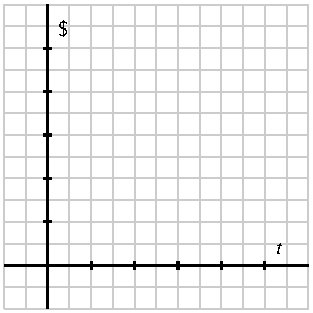
\includegraphics{growth-PA-blank-axes.pdf}
%add alt text
\end{image}
\end{enumerate}
\end{exploration}


%\typeout{************************************************}
%\typeout{Subsection 3.1.1 Exponential functions of form $f(t) = ab^t$}
%\typeout{************************************************}


\section{Exponential functions of form $f(t) = ab^t$}

In the exploration above, we encountered the functions $I(t)$ and $V(t)$ that had the same basic structure.  Each can be written in the form $g(t) = ab^t$ where $a$ and $b$ are positive constants and $b \ne 1$.  Based on our earlier work with transformations, we know that the constant $a$ is a vertical scaling factor, and thus the main behavior of the function comes from $b^t$, which we call an ``exponential function''.%
\begin{definition}
Let $b$ be a real number such that $b > 0$ and $b \ne 1$.  We call the function defined by%
$$f(t) = b^t$$
an \dfn{exponential function} with \dfn{base} $b$.%
\end{definition}

For an exponential function $f(t) = b^t$, we note that $f(0) = b^0 = 1$, so an exponential function of this form always passes through $(0,1)$.  In addition, because a positive number raised to any power is always positive (for instance, $2^{10} = 1096$ and $2^{-10} = \frac{1}{2^{10}} = \frac{1}{2096}$), the output of an exponential function is also always positive.  In particular, $f(t) = b^t$ is never zero and thus has no $x$-intercepts.

Because we will be frequently interested in functions such as $I(t)$ and $V(t)$ with the form $ab^t$, we will also refer to functions of this form as ``exponential'', understanding that technically these are vertical stretches of exponential functions according to our definition of exponential function.  In the exploration above, we found that $I(t) = 20000(1.08)^t$ and $V(t) = 20000(0.88)^t$.  It is natural to call $1.08$ the ``growth factor''  of $I$ and similarly $0.88$ the growth factor of $V$.  In addition, we note that these values stem from the actual growth rates:  $0.08$ for $I$ and $-0.12$ for $V$, the latter being negative because value is depreciating.  In general, for a function of form $f(t) = ab^t$, we call $b$ the \dfn{growth factor}. \index{exponential function!growth factor}  Moreover, if $b = 1+r$, we call $r$ the \dfn{growth rate}. \index{exponential function!growth rate}  Whenever $b > 1$, we often say that the function $f$ is exhibiting ``exponential growth'', wherease if $0 < b < 1$, we say $f$ exhibits ``exponential decay''. \index{exponential function!exponential decay}

\begin{exploration}
Suppose that at age $20$ you have \textdollar{}$20000$ and you can choose between one of two ways to use the money:  you can invest it in a mutual fund that will, on average, earn $8$\% interest annually, or you can purchase a new automobile that will, on average, depreciate $12$\% annually.  Let's explore how the $20000$ changes over time.%

Let $I(t)$ denote the value of the \textdollar{}$20000$ after $t$ years if it is invested in the mutual fund, and let $V(t)$ denote the value of the automobile $t$ years after it is purchased.

\begin{enumerate}[label=\alph*.]
\item What is the domain of $g(t) = ab^t$?
\item What is the range of $g(t) = ab^t$?
\item What is the $y$-intercept of $g(t) = ab^t$?
\item How does changing the value of $b$ affect the shape and behavior of the graph of $g(t) = ab^t$?  Write several sentences to explain.
\item For what values of the growth factor $b$ is the corresponding growth rate positive?  For which $b$-values is the growth rate negative?
\item Consider the graphs of the exponential functions $p$ and $q$ provided in teh figure below.  If $p(t) = ab^t$ and $q(t) = cd^t$, what can you say about the values $a$, $b$, $c$, and $d$ (beyond the fact that all are positive and $b \ne 1$ and $d \ne 1$)?  For instance, can you say a certain value is larger than another?  Or that one of the values is less than $1$?
\begin{image}
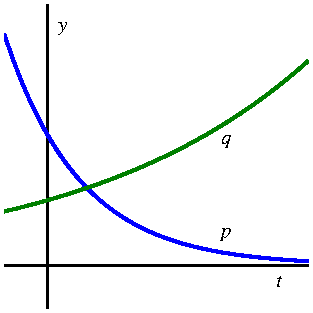
\includegraphics{growth-act-a-b-t.pdf}
%add alt text
\end{image}
\end{enumerate}
\end{exploration}
%
%\typeout{************************************************}
%\typeout{Subsection 3.1.2 Determining formulas for exponential functions}
%\typeout{************************************************}

\section{Determining formulas for exponential functions}

To better understand the roles that $a$ and $b$ play in an exponential function, let's compare exponential and linear functions.  In the tables below, we see output for two different functions $r$ and $s$ that correspond to equally spaced input.

\begin{center}
$
\begin{array}{cccccc}
%$
{\begin{array}{cc}
t&r(t)\\
\hline
0&12\\
3&10\\
6&8\\
9&6
\end{array}}&&&&&
%$
%\end{center}
%\begin{center}
%$
{\begin{array}{cc}
t&s(t)\\
\hline
0&12\\
3&9\\
6&6.75\\
9&5.0625
\end{array}}\\
\end{array}
$
\end{center}



In the leftside table for $r(t)$, we see a function that exhibits constant average rate of change since the change in output is always $\triangle r = -2$ for any change in input of $\triangle t = 3$.  Said differently, $r$ is a linear function with slope $m = -\frac{2}{3}$.  Since its $y$-intercept is $(0,12)$, the function's formula is $y = r(t) = 12 - \frac{2}{3}t$.

In contrast, the function $s$ given by rightside table for $s(t)$ does not exhibit constant average rate of change.  Instead, another pattern is present.  Observe that if we consider the ratios of consecutive outputs in the table, we see that%
\begin{equation*}
\frac{9} {12}= \frac{3}{4}, \frac{6.75}{9} = 0.75 = \frac{3}{4}, \text{ and } \frac{5.0625}{6.75} = 0.75 = \frac{3}{4}\text{.}
\end{equation*}
So, where the \emph{differences} in the outputs in the table for $r(t)$ are constant, the \emph{ratios} in the outputs in the table for $s(t)$ are constant.  The latter is a hallmark of exponential functions and may be used to help us determine the formula of a function for which we have certain information.

If we know that a certain function is linear, it suffices to know two points that lie on the line to determine the function's formula.  It turns out that exponential functions are similar:  knowing two points on the graph of a function known to be exponential is enough information to determine the function's formula.  In the following example, we show how knowing two values of an exponential function enables us to find both $a$ and $b$ exactly.

\begin{example}\label{example:exp1}
Suppose that $p$ is an exponential function and we know that $p(2) = 11$ and $p(5) = 18$.  Determine the exact values of $a$ and $b$ for which $p(t) = ab^t$.
\begin{explanation}
Since we know that $p(t) = ab^t$, the two data points give us two equations in the unknowns $a$ and $b$.  First, using $t = 2$,%
\begin{equation}
ab^2 = 11\text{,}
\end{equation}
and using $t = 5$ we also have%
\begin{equation}
ab^5 = 18\text{.}
\end{equation}
Because we know that the quotient of outputs of an exponential function corresponding to equally-spaced inputs must be constant, we thus naturally consider the quotient $\frac{18}{11}$.  Using $ab^2 = 11$ and $ab^5 = 18$, it follows that%
\begin{equation*}
\frac{18}{11} = \frac{ab^5}{ab^2}\text{.}
\end{equation*}
Simplifying the fraction on the right, we see that $\frac{18}{11} = b^3$. Solving for $b$, we find that $b = \sqrt[3]{\frac{18}{11}}$ is the exact value of $b$.  Substituting this value for $b$ in $ab^2 = 11$, it then follows that $a \left( \sqrt[3]{\frac{18}{11}} \right)^2 = 11$, so $a = \frac{11}{\left( \frac{18}{11} \right)^{2/3}}$.  Therefore,%
\begin{equation*}
p(t) = \frac{11}{\left( \frac{18}{11} \right)^{2/3}} \left( \sqrt[3]{\frac{18}{11}} \right)^t \approx 7.9215 \cdot 1.1784^t\text{,}
\end{equation*}
and a plot of $y = p(t)$ confirms that the function indeed passes through $(2,11)$ and $(5,18)$ as shown in the figure below.

\begin{image}
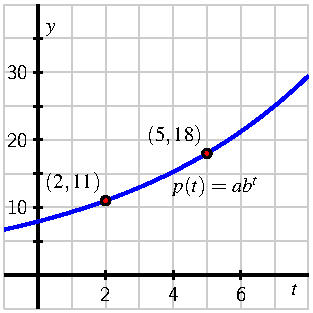
\includegraphics{growth-find-a-b.pdf}
\end{image}

\end{explanation}
\end{example}

\begin{exploration}
The value of an automobile is depreciating.  When the car is $3$ years old, its value is \textdollar{}$12500$; when the car is $7$ years old, its value is \textdollar{}$6500$.

\begin{enumerate}[label=\alph*.]
\item The value of an automobile is depreciating.  When the car is $3$ years old, its value is \textdollar{}$12500$; when the car is $7$ years old, its value is \textdollar{}$6500$.
\item The value of an automobile is depreciating.  When the car is $3$ years old, its value is \textdollar{}$12500$; when the car is $7$ years old, its value is \textdollar{}$6500$.
\item Suppose instead that the car's value is modeled by a linear function $L$ and satisfies the values stated at the outset of this activity.  Find a formula for $L(t)$ and determine both the purchase value of the car and when the car will be worth \textdollar{}$1000$.
\item Which model do you think is more realistic?  Why?
\end{enumerate}
\end{exploration}

%\typeout{************************************************}
%\typeout{Subsection 3.1.3 Trends in the behavior of exponential functions}
%\typeout{************************************************}

Recall that a function is increasing on an interval if its value always increasing as we move from left to right.  Similarly, a function is decreasing on an interval provided that its value always decreases as we move from left to right.

\begin{image}
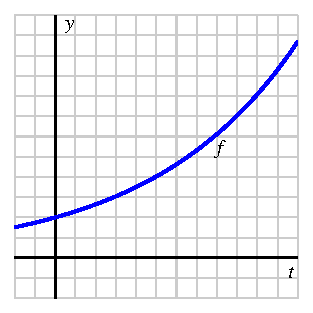
\includegraphics{growth-incr-CCU.pdf}
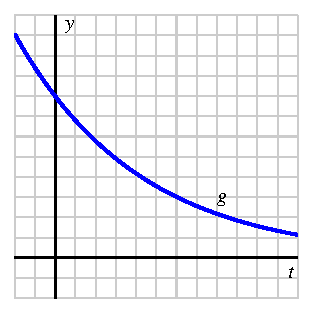
\includegraphics{growth-decr-CCU.pdf}
\end{image}

If we consider an exponential function $f$ with a growth factor $b > 1$, such as the function pictured in the left-hand graph above, then the function is always increasing because higher powers of $b$ are greater than lesser powers (for example, $(1.2)^3 > (1.2)^2$).  On the other hand, if $0 < b < 1$, then the exponential function will be decreasing because higher powers of positive numbers less than $1$ get smaller (e.g., $(0.9)^3 < (0.9)^2$), as seen for the exponential function in the right-hand graph above.

An additional trend is apparent in the graphs in above.  Each graph bends upward and is therefore concave up.  We can better understand why this is so by considering the average rate of change of both $f$ and $g$ on consecutive intervals of the same width.  We choose adjacent intervals of length $1$ and note particularly that as we compute the average rate of change of each function on such intervals,%
\begin{equation*}
AV_{[t,t+1]} = \frac{f(t+1) - f(t)}{t+1-1} = f(t+1) - f(t)\text{.}
\end{equation*}
Thus, these average rates of change are also measuring the total change in the function across an interval that is $1$-unit wide. We now assume that $f(t) = 2 (1.25)^t$ and $g(t) = 8(0.75)^t$ and compute the rate of change of each function on several consecutive intervals.


\begin{center}
$
%\begin{array}{cccccc}
%$
{\begin{array}{ccc}
\multicolumn{3}{c}{\text{The average rate of change of } f(t) = 2(1.25)^t}\\
t&f(t)&AV_{[t,t+1]}\\
\hline
0&2&0.5\\
1&2.5&0.625\\
2&3.125&0.78215\\
3&3.90625&0.97656
\end{array}}%&&&&&
$
\end{center}
\begin{center}
$
{\begin{array}{ccc}
\multicolumn{3}{c}{\text{The average rate of change of } g(t) = 8(0.75)^t}\\
t&g(t)&AV_{[t,t+1]}\\
\hline
0&8&-2\\
1&6&-1.5\\
2&4.5&-1.125\\
3&3.375&-0.84375
\end{array}}%\\
%\end{array}
$
\end{center}

From the data in the first table about $f(t)$ we see that the average rate of change is increasing as we increase the value of $t$.  We naturally say that $f$ appears to be ``increasing at an increasing rate''.  For the function $g$, we first notice that its average rate of change is always negative, but also that the average rate of change gets \emph{less negative} as we increase the value of $t$. Said differently, the average rate of change of $g$ is also increasing as we increase the value of $t$.  Since $g$ is always decreasing but its average rate of change is increasing, we say that $g$ appears to be ``decreasing at an increasing rate''.  These trends hold for exponential functions generally according to the conditions given below.  It takes calculus to justify this claim fully and rigorously. 

\begin{callout}
\section{Trends in exponential function behavior.}
For an exponential function of the form $f(t) = ab^t$ where $a$ and $b$ are both positive with $b \ne 1$,\leavevmode%
\begin{itemize}[label=\textbullet]
\item{}\hypertarget{p-1228}{}%
if $b > 1$, then $f$ is always increasing and always increases at an increasing rate;%
\item{}\hypertarget{p-1229}{}%
if $0 < b < 1$, then $f$ is always decreasing and always decreases at an increasing rate.%
\end{itemize}
\end{callout}

Observe how a function's average rate of change helps us classify the function's behavior on an interval:  whether the average rate of change is always positive or always negative on the interval enables us to say if the function is always increasing or always decreasing, and then how the average rate of change itself changes enables us to potentially say \emph{how} the function is increasing or decreasing through phrases such as ``decreasing at an increasing rate''.

\begin{exploration}

For each of the following prompts, give an example of a function that satisfies the stated characteristics by both providing a formula and sketching a graph.

\begin{enumerate}[label=\alph*.]
\item A function $p$ that is always decreasing and decreases at a constant rate.
\item A function $q$ that is always increasing and increases at an increasing rate.
\item A function $r$ that is always increasing for $t < 2$, always decreasing for $t > 2$, and is always changing at a decreasing rate.
\item A function $s$ that is always increasing and increases at a decreasing rate.  (Hint: to find a formula, think about how you might use a transformation of a familiar function.)
\item A function $u$ that is always decreasing and decreases at a decreasing rate.

\end{enumerate}

\end{exploration}

\begin{summary}\begin{itemize}
\item We say that a function is exponential whenever its algebraic form is $f(t) = ab^t$ for some positive constants $a$ and $b$ where $b \ne 1$.  (Technically, the formal definition of an exponential function is one of form $f(t) = b^t$, but in our everyday usage of the term ``exponential'' we include vertical stretches of these functions and thus allow $a$ to be any positive constant, not just $a = 1$.)
\item To determine the formula for an exponential function of form $f(t) = ab^t$, we need to know two pieces of information.  Typically this information is presented in one of two ways.
\begin{itemize}
\item If we know the amount, $a$, of a quantity at time $t = 0$ and the rate, $r$, at which the quantity grows or decays per unit time, then it follows $f(t) = a(1+r)^t$.  In this setting, $r$ is often given as a percentage that we convert to a decimal (e.g., if the quantity grows at a rate of $7$\% per year, we set $r = 0.07$, so $b = 1.07$).
\item If we know any two points on the exponential function's graph, then we can set up a system of two equations in two unknowns and solve for both $a$ and $b$ exactly.  In this situation, it is useful to consider the quotient of the two known outputs, as demonstrated in Example \ref{example:exp1}.
\end{itemize}
\item Exponential functions of the form $f(t) = ab^t$ (where $a$ and $b$ are both positive and $b \ne 1$) exhibit the following important characteristics:
\begin{itemize}
\item The domain of any exponential function is the set of all real numbers and the range of any exponential function is the set of all positive real numbers.
\item The $y$-intercept of the exponential function $f(t) = ab^t$ is $(0,a)$ and the function has no $x$-intercepts.
\item If $b > 1$, then the exponential function is always increasing and always increases at an increasing rate.  If $0 < b < 1$, then the exponential function is always decreasing and always decreases at an increasing rate.
\end{itemize}
\end{itemize}\end{summary}



\end{document}
